\chapter*{Wstęp}
\addcontentsline{toc}{chapter}{Wstęp}
    
    % Celem pracy było zaimplementowanie emulatora procesora Ziloga Z80, dzięki któremu użytkownik mógłby w łatwiejszy sposób poznać jego architekturę.
    
    Celem pracy było zaimplementowanie emulatora procesora Zilog Z80. Emulator to program komputerowy, który duplikuje zachowania systemu komputerowego, za pomocą innego system komputerowego. \cite{studyofthetechniquesforemulationprogramming}
    W tym przypadku platformą docelową jest maszyna wirtualna Javy.
   %  W tym przypadku naśladowanym jest procesor Zilog Z80, a platformą docelową maszyna wirtualna javy.
    
	Procesor Zilog Z80 był bardzo popularny na rynku mikroprocesorów\cite{karczmarczuk}. 
	Stał się dostępny na rynku w~roku 1976 i~szybko zaczął być powszechnie stosowany w 8-bitowych systemach.
	
	Jedną z~przyczyn jego sukcesu, jest łatwy sposób sprzęgania go z innymi urządzeniami, szczególnie z kontrolerami pamięci. Inną jego zaletą jest lista rozkazów zgodna z~popularnym w tamtym czasie procesorem Intel 8080, co umożliwia uruchamianie programów napisanych pierwotnie dla tego procesora \cite{karczmarczuk}.
	
	Urządzenie to, mimo zalet, ma również poważne wady. Jego wewnętrzna budowa jest złożona jak na procesor ośmiobitowy. Piny magistrali danych nie są ułożone w logiczny sposób. Ich kolejność, jak ukazuje rysunek \ref{img:z80wyprowadzenia} (piny $D_{1} - D_{7} $) jest w losowej kolejności.
    
	\begin{figure}[h]
		\centering
		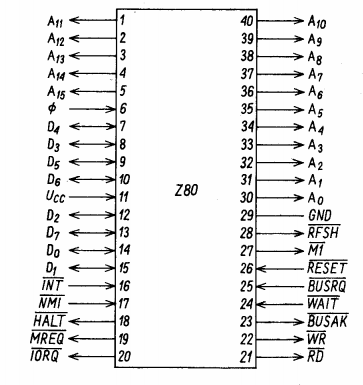
\includegraphics[width=0.5\textwidth]{z80wyprowadzenia}
		\caption{Wyprowadzenia mikroprocesora Z80 \cite{karczmarczuk}}
		\label{img:z80wyprowadzenia}
	\end{figure}
			
	
	\newpage
	Lista rozkazów procesora składa się z 158 pozycji, w tym 78 z nich jest zgodnych z~Intel 8080\cite{manual}. Poznanie działania każdego z nich jest trudne i czasochłonne dla większości osób. Omawiany projekt emulatora ma na celu, oprócz samego wykonywania kodu programu, prezentować zmiany jakie zachodzą wewnątrz procesora. Użytkownik może prześledzić proces wykonywania dowolnej instrukcji i sprawdzić jak wpływa ona na~pamięć, rejestry, czy flagi procesora. Wszystkie te wewnętrzne parametry można modyfikować podczas procesu emulacji, za pomocą graficznego interfejsu użytkownika, zaprezentowanego w~rysunku \ref{img:z80Gui}.
	
	W rozdziale pierwszym opisano proces emulacji oraz trzy sposoby jej wykonania, z~naciskiem na metodę wybraną w projekcie.
	
	Rozdział drugi zawiera przegląd wybranych emulatorów Zilog-a Z80. Skupiono się głównie na aplikacjach zawierających graficzny interfejs użytkownika tak jak opisywany projekt. 
    
    %@todo dokładniej opisać co przedstawia projekt aplikacji
    Rozdział trzeci przedstawia projekt aplikacji, wymagania funkcjonalne i niefunkcjonalne, oraz podział na moduły.
	
	Rozdział czwarty opisuje implementacje poszczególnych modułów projektu. Wyjaśniono sposób wykonywania emulacji, realizacje operacji bitowych, oraz sposób integracji poszczególnych części aplikacji.
	
	
	W rozdziale szóstym zawarto informacje na temat testów jednostkowych i manualnych aplikacji użytych w celu sprawdzenia poprawności wykonywania emulacji.
	
	W rozdziale siódmym podsumowano projekt oraz opisano ewentualne możliwości rozwoju.